\documentclass[10pt]{article}
\newcommand{\HRule}{\rule{\linewidth}{0.5mm}}
\parindent 0pt
\parskip 10pt
\usepackage{anysize}
\usepackage{graphicx}
\usepackage{epsfig}
\usepackage{float}
%\usepackage{cite}
\usepackage{natbib}
\usepackage{setspace}
\marginsize{3.5cm}{3.5cm}{1cm}{1cm}
\onehalfspacing
\usepackage{caption}
\usepackage{subcaption}
\usepackage{amsmath,hyperref}

\usepackage{xcolor}
\hypersetup{
    colorlinks,
    linkcolor={red!50!black},
    citecolor={blue!50!black},
    urlcolor={blue!80!black}
}

%\textwidth 15cm
%\textheight 24cm
%\onehalfspacing
\begin{document}

\title{Classification Algorithm Comparisons: Mine Detection Study}

\author{David Starkey}

\maketitle





\section{Mine Detection: Introduction and Data Source}

An important application of Sonar for underwater vehicles is in identifying harmful objects from background underwater debris. This data set \footnote{\href{ https://archive.ics.uci.edu/ml/datasets/Connectionist+Bench+(Sonar,+Mines+vs.+Rocks)}{\textcolor{blue}{https://archive.ics.uci.edu/ml/datasets/Connectionist+Bench+(Sonar,+Mines+vs.+Rocks)}}} records the magnitude of the reflected response in 60 frequency bands when bounced off a set of underwater targets. 111 of these patterns are obtained by the reflected signal bounced off rocks, and a further 97 patterns are returned from mines. A simple diagram illustrating the sonar classification problem is presented in Figure \ref{fig_diag}. The analysis and discussion presented in this work aims to:

\begin{itemize}
\item Classify the return sonar signals as 'Mine Detection' or 'Rock Detection'.

\item Test various classification machine learning algorithms against each other using a cross validation approach to measure classification accuracy. The classifiers used include a multi-layer neural network, k-nearest neighbour, k-means clustering and a random forest decision tree classifier.

\item Measure the computation efficiency of each of the above classification approaches.

\end{itemize}


In the sections that follow, four classification approaches will be introduced. Relevant theory and algorithms discussed and a comparison of each classifiers performance presented.

\begin{figure}
\begin{center}
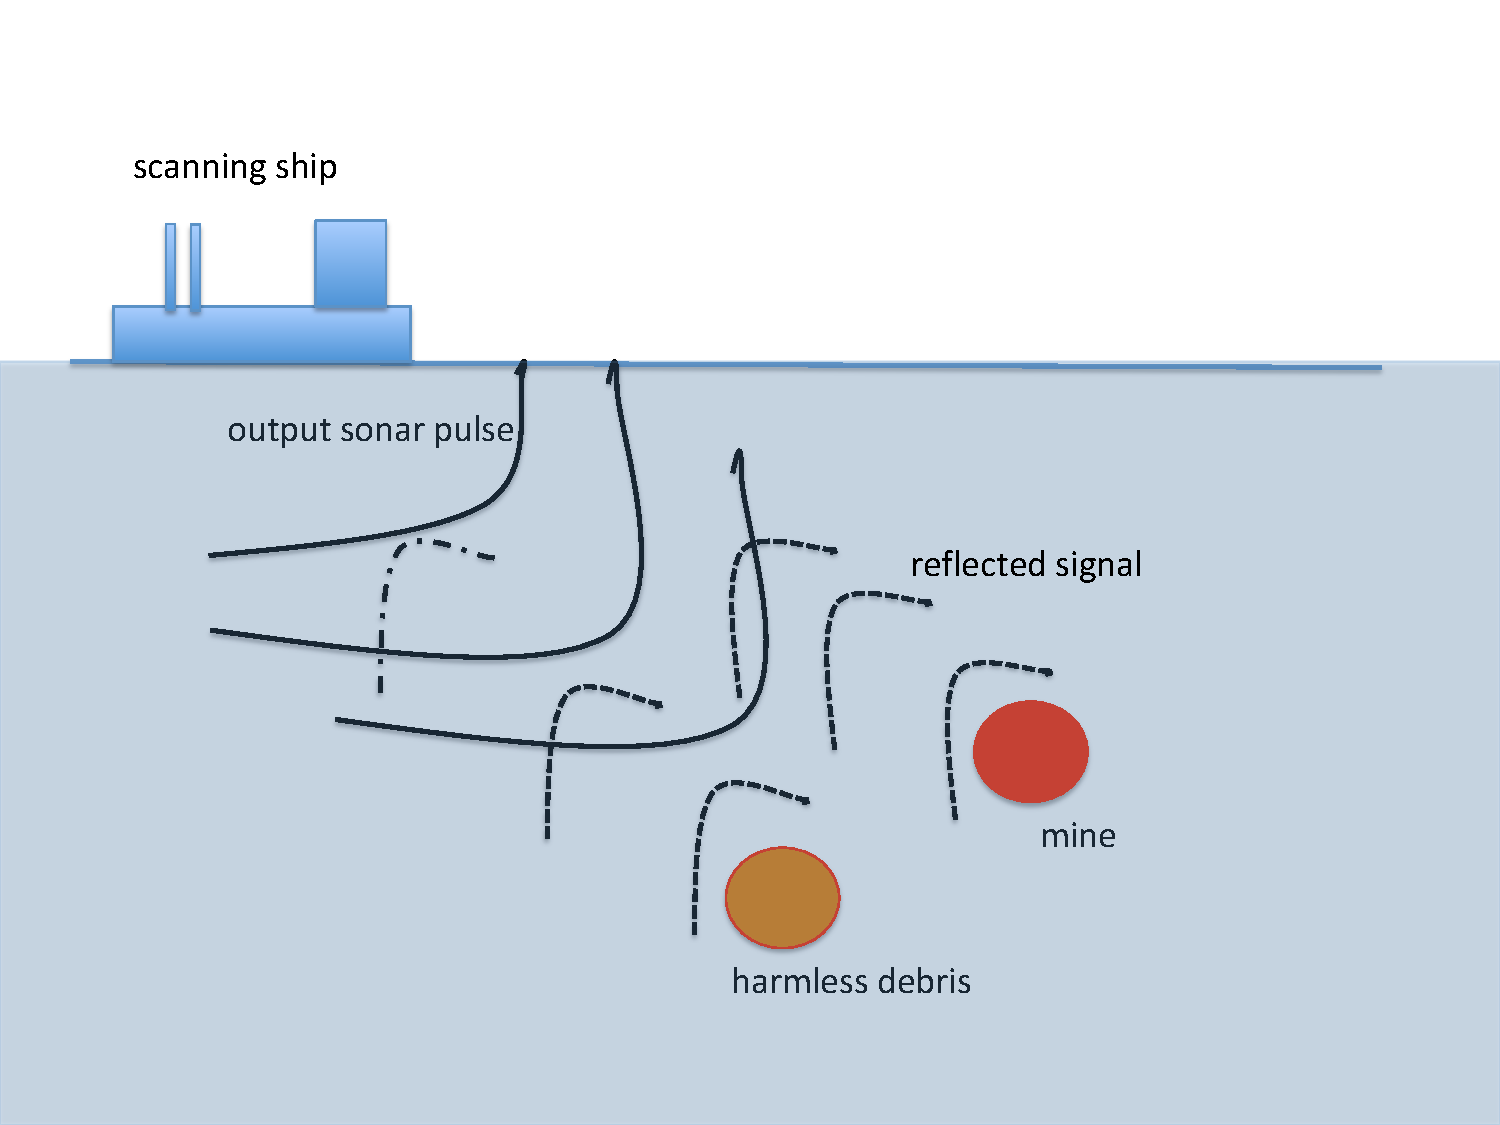
\includegraphics[scale=0.6,angle=0,trim=2cm 0cm 0cm 2cm]{sonar_diagram.pdf}
\caption{Diagram of the sonar classification experiment. A reflected signal from a multi-band output pulse must be interpreted and the origin of the reflected echo must be classified as `mine' or `not a mine'. }
\label{fig_diag}
\end{center}
\end{figure} 




\section{K-nearest neighbour algorithm and classification}
The first machine learning method used to classify the mine data is known as k-nearest-neighbour. The algorithm can be summarised as follows:

\begin{itemize}
\item for each example $\vec{X_i}$ in the test dataset, calculate the euclidean distance to every $j$th point $\vec{y_j}$ in the training sample. For an $l$ dimensional dataset, this is 
\begin{equation}
d_{ij} = \sqrt{\left( \sum_l X_{il} - y_{jl} \right)^2}.
\label{eq_euclid}
\end{equation}

\item From the above quantities, identify the k ($k = 3$ is chosen for this work) closest points to data point $\vec{X_i}$ and calculate the mode classification of these $k$ closest points in the training set.

\item assign this classification to the test point $\vec{X_i}$ and repeat for the remaining examples.


\end{itemize}


K-nearest-neighbour is a simple but robust machine learning classification algorithm. One can avoid over-fitting to noise in the training data by choosing a suitably large value of k such that a rogue point in the training data is down weighted by the remaining of the $k-1$ points adjacent to $\vec{X_i}$ when calculating the mode classification.








\section{Hidden-Layer Neural Network}
\label{sec_nn}

Neural networks are slightly more difficult algorithms to understand theoretically but have the advantage that, once trained on a training sample, are faster at classifying new test examples than a K-nearest neighbour method.  The section below will outline the theory of a single layer neural network before developing this to a neural network with a hidden layer. The interested reader is advised to consult XX that offers an excellent in-depth discussion of the required, linear algebra, calculus and statistics involved in all steps of the back propagation algorithm used to train a neural network.

\subsection{Theory} 


In its simplest form, a neural network is composed of a single ($j=1$) `neuron'. This neuron takes an arbitrary number of $i$ input values, each modulated by a `weight' parameter $W_{ij}$ \footnote{Much of the theory in this section can be found in most texts on neural networks but wikipedia does a good job explaining the mathematical detail \href{ https://en.wikipedia.org/wiki/Backpropagation}{\textcolor{blue}{https://en.wikipedia.org/wiki/Backpropagation}}, as do the online Stanford lecture series' \href{ https://www.coursera.org/lecture/machine-learning/backpropagation-algorithm-1z9WW}{\textcolor{blue}{https://www.coursera.org/lecture/machine-learning/backpropagation-algorithm-1z9WW}}}. The weighted sum of these is known as the `activation' $z$ and is operated on by the neuron with an activation function $f (z)$ to yield an output quantity $a$. The output from the entire neural network for an input data example vector $\vec{X}_n$ (in situations with a chain of neurons as is the case later) is denoted $h(W,\vec{X}_n)$. A back propagation approach is used to optimize the weights (detailed below) in multi layer neural networks. This requires that the activation function $f(z)$ be differentiable. In this project (as is common for many neural networks), a sigmoid activation function is adopted where 

\begin{equation} 
f(z) = \frac{1}{1+e^{-z}},
\label{eq_sigmoid}
\end{equation}

\noindent with a derivative

\begin{equation} 
f`(z) = f(z) \left( 1 - f(z) \right).
\label{eq_sigmoid}
\end{equation}


\noindent This activation function always returns a number between 0 and 1. Once the weights are optimised, the neuron will output a value close to 0 to indicate one class, and close to 1 to indicate the other. The mathematical rigour in neural networks is in the weight-optimisation step. 







\subsection{optimizing the weights}

Like many optimisation problems, I start with the cost function (often called $\chi^2$ or the error function). For a single (or multi) layer neural network, this takes the form.

\begin{equation}
J(W) = \frac{1}{N} \sum_{n=1}^N \frac{ \left( h(W,\vec{X}_n) - y_n \right)^2} {2}
\label{eq_cost}
\end{equation}

\noindent where $y_n$ denotes the classification of the $n$th training sample of $N$ total samples with an input data vector $\vec{X}_n$.



The back propagation algorithm works using the principle of gradient descent. This iteratively updates each weight until the cost function is minimised. After one iteration, the weight $W_{ij}$ is adjusted according to 

\begin{equation}
W_{ij} = W_{ij} - \alpha \frac{\partial}{\partial W_{ij}} J\left( W \right),
\label{eq_adjust_w}
\end{equation}



\noindent where $\alpha$ is the learning rate. A high value $>1$ for the learning rate will encourage the weight parameter to take large steps as it is optimized. This has the potential advantage of reducing the convergence time but may cause the global minimum to be missed and lead inaccurate weights.

The partial derivative of the total cost function $\frac{\partial}{\partial W_{ij}} J\left( W \right)$ depends on the partial derivatives of each of the $N$ training examples like 

\begin{equation}
\frac{\partial}{\partial W_{ij}^{(l)}} J(W,b) = \left[ \frac{1}{N} \sum_{i=1}^N \frac{\partial}{\partial W_{ij}^{(l)}} J(W; \vec{x_i}, y_i) \right], 
\label{eq_partial_tot}
\end{equation}


\noindent and the partial derivatives for the individual weight parameters $\frac{\partial}{\partial W_{ij}^{(l)}} J(W; \vec{x_i}, y_i)$ are given by 



\begin{equation}
\frac{\partial}{\partial W_{ij}} J\left( W \right) = a_j^l \delta_i^{l+1},
\label{eq_partdiv}
\end{equation}

\noindent where $a_j^l$ corresponds to the output from neuron $j$ in level $l$. The intermediate error function $\delta_i^{l+1}$ calculates how responsible the $i$th neuron in layer $l$ is for errors in the output. $\delta$ depends on the level of the neuron in the network. For an outer level neuron in layer $l=n_l$,

\begin{align}
\delta^{(n_l)}_i
= \frac{\partial}{\partial z^{(n_l)}_i} \;\;
\frac{1}{2} \left\|y - h_{W,b}(x)\right\|^2 = - (y_i - a^{(n_l)}_i) \cdot f'(z^{(n_l)}_i),
\label{eq_delta}
\end{align}


\noindent and for an inner level neuron

\begin{equation}
\delta^{(l)}_i = \left( \sum_{j=1}^{s_{l+1}} W^{(l)}_{ji} \delta^{(l+1)}_j \right) f'(z^{(l)}_i).
\label{eq_delta_in}
\end{equation}


Combining Equations \ref{eq_partial_tot} through \ref{eq_delta_in} with Equation \ref{eq_adjust_w} and iterating will encourage the weights toward their optimal values and minimize the cost function (Equation \ref{eq_cost}).



\section{K-means clustering}
Clustering algorithms aim to identify clusters of points in a multi-dimensional parameter space. each cluster corresponds to a particular class and the algorithm, once trained on the 60 dimensional sonar pattern space, aims to identify two clusters in the data space. One cluster will corresponds to the signals identifying a mine and the other for signals corresponding to rocks. There are many K-means clsuter algorithms to choose from. Here a Lloyds algorithm is used. The algorithm works as follows.

\begin{itemize}
\item Arrange the dataset into a matrix $X(N,M)$ where each of the $N$ rows corresponds to one example in and $M$ dimensional feature space.

\item Normalise this matrix so each of the dimensions runs from $0$ to $1$.

\item Chose the $k$ first data points. $k$ is chosen as the number of classifications to look for. In this case $k=2$ (the signal either detects a mine or it doesn't).

\item The $k$ points will serve as the first `guess' of the cluster centroids. For each point in the training set compute which of the $k$ cluster centroids has the shortest Euclidean distance and assign it to that centroid.

\item For the set of points assigned to each cluster centroid ($n \in \j$), calculate an updated centroid position for each dimension $m$ using

\begin{equation}
C_m (j=1,k) = \frac{1}{N_j}\sum_{n \in j} X_{nm}.
\label{eq_km_update}
\end{equation}

\item Repeat until convergence.

\end{itemize}



\section{Random Forest Decision Tree Classifier}
\label{sec_rf}


The random forest decision tree classifier is a rather complex algorithm with many steps. A disadvantage to this algorithm (as will become apparent after following the steps below) is that it has a large number of tunable `hyper parameters' that must be set for the decision tree to work. While more simple algorithms like $k$ means clustering are very direct with no `tune-ing' requirements, a random forest requires the user to specify the number of trees in the forest, the depth of each tree, the cost function and in some cases the method by which to assign the class (i.e should we average the probability distributions from each tree or use the mode class from each tree to assign the class). Despite this draw back, however, random forest classifiers are very visual classifiers for a general audience to understand intuitively even if the full details of the algorithm are unclear. They are also quite robust and provide very accurate classifications in general. The algorithm for creating a single tree is as follows:

\begin{itemize}
\item Arrange the dataset into a matrix $X(N,M)$ where each of the $N$ rows corresponds to one example in and $M$ dimensional feature space. Also arrange the classes into an array $C(M)$. These should ideally take numerical values from $1$ up to the number of distinct classes (e.g 1 or 2 in this case).


\item Consider a random set of $K < M$ dimensions in the parameter space and a random subset of $I<N$ points from the data set. 

\item We now need a value $S$ above and below which to split the $I$ considered points. The value of all $I$ points, in each dimension $k \in K$ are considered in turn as the split point $S$.

\item Identify the number of points that lie either side (e.g $N_{l=1}$ points below and $N_{l=2}$ points above) of the current-considered point $i$ in the subset of $I$, in the current-considered dimension $k$ in the subset of $K$ (e.g $N_l$ where $X(I,k) < S$). This will be a split in the decision tree. The probability $w_l$ of finding a point in the subset of $I$ either side of the split (known as a `branch') is given by $w_l=N_l/M$.

\item For each branch $l$ in the split, calculate the square probability of finding a class label $j$ (`mine' or `no mine') in the branch (in this case $N_j=2$ corresponding to each of the $N_j$ classes). Sum this and subtract from 1.

\begin{equation}
G_l = 1 - \sum_{j=N_j}p_j^2.
\label{eq_gini1}
\end{equation}

The Cost function for a given split of a node is then the Gini index, given by summing the coefficient $G_l$ over all the $l$ branches weighted by the probability of finding the object in the branch $w_{l}$,

\begin{equation}
\label{eq_gini}
I_G(p) = \sum_{l=1}^{N_l} w_{l} G_{l}.
\end{equation}

\noindent Here $N_l$ is always two (there are always two branches to each tree as we are splitting points as being either above or below a given split $S$. The choice of split $S$ is given by considering, in turn, each point in the subset of $I$ rows and $K$ dimensions as the split $S$. The value of the data matrix that minimises the Gini index is chosen as the split point $S = X(i,k)$.


\item The previous point, $I_G (p)$, computes the split for a given node. Repeat this for each child of the above node and continue to deepen the tree up to a desired depth (e.g 5 levels). Each time a new node is considered, chose a new random set of $K$ dimensions and $I$ points to consider for the split quantity. The choice of depth is somewhat arbitrary but the node path terminates once the tree has reached a certain depth or if there are no children in the branch following a split (no more data left to populate the branch).

The above algorithm generates a single decision tree. The random forest algorithm works by constructing an arbitrary number of trees (e.g 5, 10, 50) and propagating new test data through each tree. The terminal node of each tree produces a probability distribution of the new test data belonging to a particular class. An average probability distribution is computed using the results of each tree of the forest and this is used to assign the class of the test data.

\end{itemize}






\section{Dimensionality Reduction Using PCA}
Principal Component Analysis (PCA) aims to reduce the dimensionality of a dataset by defining a new co-ordinate system (with fewer dimensions than the original dataset) whose principal axes lie along the direction of largest variance of the data. For classification problems, this allows the user to eliminate irrelevant information and focus the classification machine learning algorithm on the data in the new (lower dimensional) co-ordinate system.

The steps of a PCA algorithm are outlined as follows:
\begin{itemize}
\item organize the input dataset as a matrix with $N$ columns corresponding to the number of test samples, and $m$ rows corresponding to the dimensionality of the input data. This is the data matrix $X_{nm}$.

\item Calculate the mean of each of the $m$ dimensions and subtract this off. The new matrix is now $X`_{nm}$

\item Compute the covariance of $X`_{nm}$.

\item Compute the eigenvectors and eigenvalues of the covariance matrix.

\item The eigenvectors now define the principal components. The magnitude of the eigenvalues corresponds to the amount of variance along the new co-ordinate axis. 'Eigenvector one' corresponds to the principal component axis containing the largest portion of the variance. 

\end{itemize}


A sub-sample (fewer than $m$) of eigenvectors (from high-to-low eigenvalues)  can now be selected to capture the interesting variability of the data without the need to use the full $m$ dimensions of the input data. Depending on the specific problem, applying PCA before performing a machine learning classification can significantly speed up the training process without significant loss of accuracy. 





\section{Results}

This comparison between the 4 classification methods above will investigate the accuracy and computation efficiency (or time) of each method. The first attribute to compare is the accuracy of the classification. A cross validation approach is applied to the data set where a sub-sample of ten random points are subtracted from the sonar dataset to serve as the test data. The accuracy can then be assessed as the ratio of the number of correctly classified points to the total number of test points in the sub-sample. To test the accuracy improvement with sample size, I resample the training data. A sub-sample of size N is extracted from the training data and the classification algorithms retrained on this sub-sample. The accuracy is assessed for each machine learning classifier as a function of sub-sample size N where N increases from 10 percent to 100 percent of the original sub-sample. 

Figure \ref{fig_acc} shows the improvement with sub sample size for the various classifier algorithms. It is clear that sample size tends to improve classifying accuracy for all the classifying techniques, with the most dramatic improvement found in the random forest classifier which improves from 65\% to 90\% as the sample size is increased from the lowest to the maximum size. The worst performing classification technique appears to be the K-means clustering approach. K-means clustering, while a very useful and simple clustering algorithm, is not always effective as a classifier. Clustering algorithms do not utilize the 'class' information of the training data sample. They simply note how many classes to look for and iteratively find the centroids for the clusters. This works well if data is separated into distinct regions or 'blobs' in the attribute parameter space. In practise this may not be the case. The algorithm can also easily be confused in higher-dimensional probability spaces (here we have 60 unique signals at various frequencies to consider). The neural net and random forest classifiers perform much better for this particular problem and note the best improvement with increasing training sample size. The K-neaerest neighbour approach also notes consistent improvement with increasing sample size and approaches 80\% accuracy when trained on the maximum sample. 

The second attribute compared in this analysis is the computation time. Often we require efficient classifiers that work on low to modest level CPU's. These may be small and required to operate on mobile devices which lack the high computational power of a desktop machine or cluster. Figure \ref{fig_comptime} summarizes the computation times. The training stage of machine learning algorithms like neural nets is often performed prior to testing on more remote devices. Therefore only the forward propagation computation time for the test data is counted here. It can be seen that the neural net is the fastest of the four algorithms tested by a dramatic margin (around 100 times faster than the decision tree random forest classifier used here). The decision tree random forest, while accurate, appears to be the slowest. One caveat to note here is that both neural nets and random forest decision trees have a large number of tune-able parameters (or hyper parameters) that need to be specified to construct the tree or neural net. These include the maximum tree size, the number of hidden layers in the network and the number of neurons in each layer. One therefore should attempt several different network or tree configurations to decide which offers the best balance between accuracy and computation time.



\begin{figure}
\begin{center}
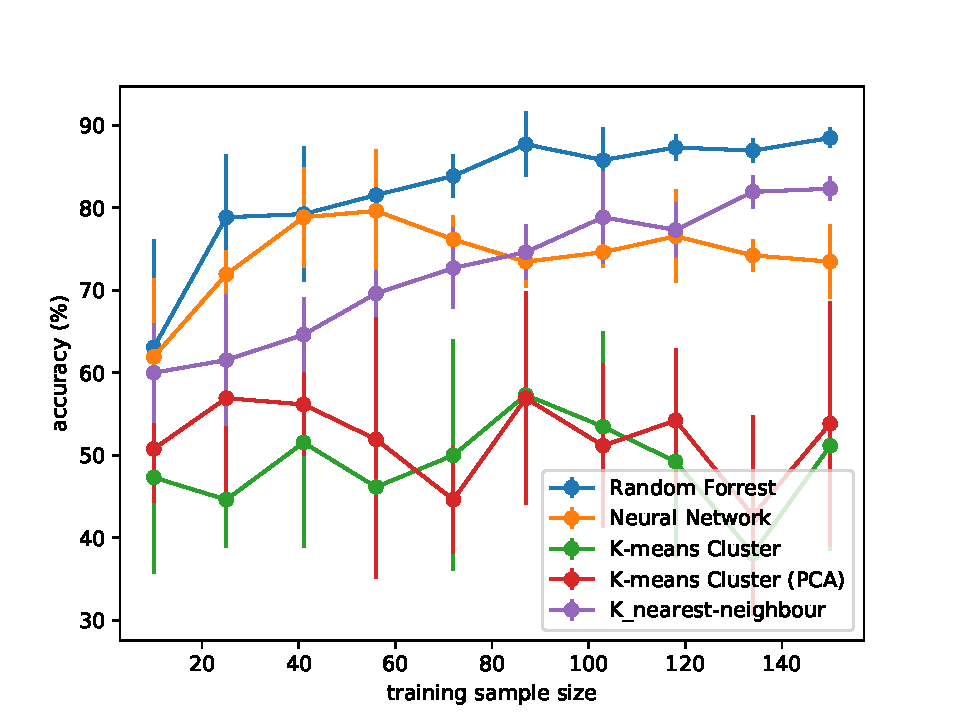
\includegraphics[scale=1.0,angle=0,trim=0cm 0cm 0cm 0cm]{comparison_accuracy.pdf}
\caption{Performance test for the four classification techniques vs training sample size. The classification accuracy is shown on the y axis where the error bars indicate the rms classification accuracy from five independent tests.}
\label{fig_acc}
\end{center}
\end{figure} 




\begin{figure}
\begin{center}
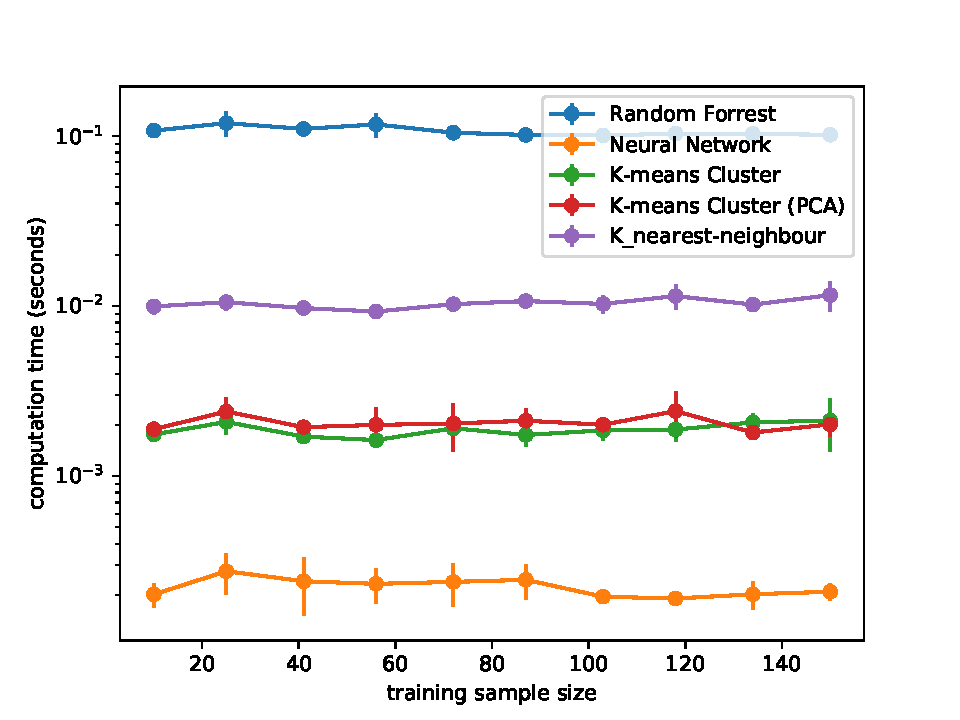
\includegraphics[scale=1.0,angle=0,trim=0cm 0cm 0cm 0cm]{comparison_time.pdf}
\caption{Performance test for the four classification techniques vs training sample size. The computation time (minus the training time) is shown on the y axis where the error bars indicate the rms computation time from five independent tests.}
\label{fig_comptime}
\end{center}
\end{figure} 





Some specific general advantages and disadvantages of the four methods are discussed below.

\subsection{Neural net (Multi-layer Perceptron}
An example neural net configuration for the classification problem is shown in Figure \ref{fig0} where colours represent the weights optimized during the training.


\subsubsection{Advantages}
\begin{itemize} 

\item among the most accurate of the machine learning algorithms for this data.

\item Once trained, very fast to compute for new test data. 

\end{itemize}




\subsubsection{Disadvantages}
\begin{itemize} 

\item Many tunable parameters can sometimes require extensive trial and error approach to determine the optimum layout of the network.

\item Often requires regularisation methods to avoid over-fitting (weight decay terms etc).

\item Once trained, very fast to compute for new test data. 

\end{itemize}




\subsection{Random Forest Decision Tree}
Decision tree random forest construct many trees based. To classify a new test data point. Each tree is traversed in turn. Each node asks a specific question about one of the attributes of the test data and (for binary trees) the data either splits to the left or right branch depending on the answer. The questions are set by minimising a quantity called the Gini index (See section \ref{sec_rf}). The relative numbers of training points at the termination point give rise to a posterior probability distribution to assign the class of the new data point. In a forest, the average posterior distribution is used to classify the new data. A sample decision tree from the mine classification data is shown in Figure \ref{fig_dt}.


\begin{figure}
\begin{center}
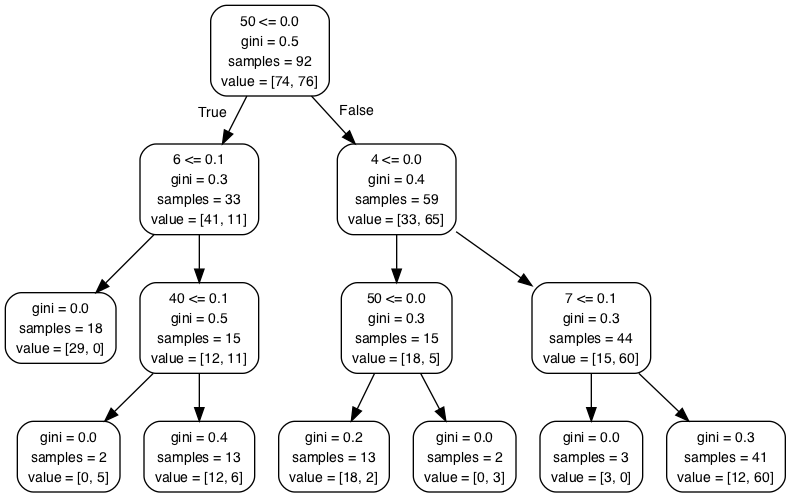
\includegraphics[scale=0.6,angle=0,trim=3cm 0cm 0cm 0cm]{small_tree_9_0.png}
\caption{A sample decision tree in the random forest classifier. The full tree sizes are too large to be viewed easily so a smaller tree is presented here as a conceptual aid. Each node (box) is annotated with three lines. The first shows the attribute number in question. With an inequality indicating the split inequality (e.g the first node states 'If the signal strength of the sonar signal in the 50th frequency band is less than or equal to zero, take the left branch. Else take the right branch). The second line shoes the value of the Gini coefficient (Section \ref{sec_rf}). The fourth line shows the number of training data in this node the went down either the left or right branch and the third line shows the number of sub-sampled points used to construct the split point in the first line.}
\label{fig_dt}
\end{center}
\end{figure} 


\subsubsection{Advantages}
\begin{itemize} 

\item For the full sample size, the random forest classifier proved the most accurate of the machine learning algorithms for this data.

\item Very intuitive to visualise. It is easy to understand making decisions attribute-by attribute and following the tree to its end. A neural net on the other hand is less conceptually obvious to understand by viewing the network as all the neurons talk to those on previous and subsequent layers. I.e all the parameters are involved in setting the weights for each neuron, unlike the decision tree.

\end{itemize}




\subsubsection{Disadvantages}
\begin{itemize} 

\item Many tunable parameters can sometimes require extensive trial and error approach to determine the optimum layout of the network.

\item Among the slowest classifier used in the sonar mine data project

\end{itemize}









\subsection{K-means clustering}
K-means algorithms failed spectacularly to classify the mine data for this experiment. This is partly because the clustering patterns of points to which K-means is sensitive is not always obeyed. One can imagine two distinct blobs in a 2D attribute space, one for each class, where K-means correctly identifies attribute clusters and assigns class labels appropriately. If faced with a different arrangement of points, perhaps an inner blob belonging to one class that is surrounded by a ring of points belonging to a second class, both classes would have the same cluster centre and the K-means algorithm would fail to classify new data points. K-means can easily be tricked in this way and is not always ideal to use as a classifier. It is included here only for completeness.




\subsection{K-nearest neighbour}
K-nearest neighbour is the simplest classification algorithm to code and understand. In this experiment it performed on par with the more sophisticated neural net and random forest classifiers albeit requiring more time to classify the test data than the neural network. 

\subsubsection{Advantages}
\begin{itemize}
\item Simple to code and understand.

\item Few hyper-parameters (tune-able settings) make the code robust to implement.

\item High performance (> 80\%) success rate at identifying mines from the sonar data.

\end{itemize}



\subsubsection{Disadvantages}
\begin{itemize}
\item High computation time (>10 times slower than the neural network classifier).


\end{itemize}

 
%is extracting a sample size increasing from zero to one-hundred percent of the original training sample size (with the test data already extracted). The accuracy of both K-nearest-neighbour and the neural network as a function of training sample size are compared in Figure xx. The figure also shows that reducing the dimensionality of the parameter space using PCA slightly reduces the accuracy of the neural network and K-nearest neighbour algorithm. The effect is most dramatic for the neural network, however even with PCA-reduced parameter space, the neural network consistency outperforms the K-nearest neighbour algorithm for all sample sizes. The variability along the two dimensions of highest variance (PCA eigenvector 1 and 2) are plotted in Figure xx.

%The computation speeds of the neural net method and the K-nearest neighbour approach are shown in Figure xx. Note that the K-nearest-neighbour algorithm does not contain a specific training step. The full algorithm must be computed for every new test point.  The neural net on the other hand can be split into a training and a test step. Once trained, any new data need only be propagated through the already-trained algorithm. Figure xx therefore presents the training and testing steps of the neural network separately. Figure xx shows that the combined training and testing steps of the neural network are significantly higher than the compute time for K-nearest-neighbour. Once trained however, the neural network is able to classify new data much faster than the K-nearest neighbour algorithm; by factors of around three across all sample sizes. It can also be seen that for this data set, PCA does not significantly reduce the computation time. This may be because the original data set was only 5 dimensional (four independant variables and one class variable). For higher dimensional datasets, PCA may offer a more dramatic improvement on computation time with only a slight reduction in accuracy. Future data projects in the series will examine higher dimensional data sets to investigate this further.


\begin{figure}
\begin{center}
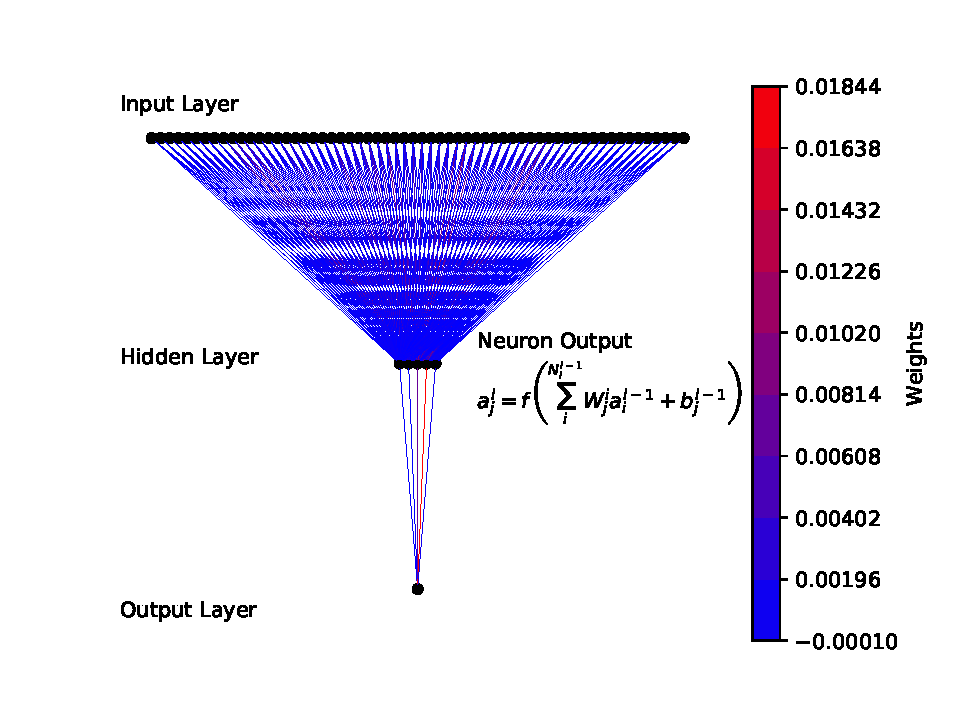
\includegraphics[scale=1.3,angle=0,trim=3.5cm 1cm 0cm 0cm]{nnplot_0_1.pdf}
\caption{An example neural network fitted to the sonar mine data. The top (input) layer contains the input signal strengths for each of the 60 rf channels. This is propagated to a hidden layer that contains five neurons. The outputs from this hidden layer are then combined and fed into the output layer to yield the output class. The colour bar shows the strengths of individual weights indicated by the line connecting two neurons. The fit also includes a bias signal for each layer that is added to the weighted sum of the input signals to each neuron prior to computing the activation function (see Section \ref{sec_nn}).}
\label{fig0}
\end{center}
\end{figure} 


\section{Conclusions}
A cross validation study was performed to compare the performance accuracy and computation time of four classification algorithms and applied to sonar signal data to distinguish mines from underwater debris. The four methods compared were the K-nearest neighbour classifier, random forest decision tree, multi-layer-perceptron and a K-means clustering algorithm. The main findings are summarized below. 
\begin{enumerate}
\item Both the random forest, neural network and K-nearest-neighbour classifiers achieved > 80\% sucess rate at classifying mines when trained on the full training data set.

\item The K-nearest neighbour classifier performed poorly. Having been confused by the large dimensionality of the attribute parameter space (60 attributes). A PCA algorithm was used to reduce this parameter space but failed to improve the performance of the K-nearest neighbour approach.

\item The computation time proved relatively fast for all methods. The neural network was significantly faster than the other methods (once trained) and achieved sub-millisecond classification time for all sample sizes.

\item The decision tree random forest classifier proved the most accurate classification method (achieving 90\% classification accuracy with the largest training size) , but also the slowest with an average computation time around one tenth of a second.
\end{enumerate}



Further comparison experiments are available and document in this github link \footnote{\href{ https://github.com/dstarkey23/projects}{\textcolor{blue}{https://github.com/dstarkey23/projects}}} with more classification tests on a variety of datasets expected presently. 
\end{document}



